% Options for packages loaded elsewhere
\PassOptionsToPackage{unicode}{hyperref}
\PassOptionsToPackage{hyphens}{url}
\PassOptionsToPackage{dvipsnames,svgnames,x11names}{xcolor}
%
\documentclass[
  10,
  a4paper,
]{article}

\usepackage{amsmath,amssymb}
\usepackage{lmodern}
\usepackage{iftex}
\ifPDFTeX
  \usepackage[T1]{fontenc}
  \usepackage[utf8]{inputenc}
  \usepackage{textcomp} % provide euro and other symbols
\else % if luatex or xetex
  \usepackage{unicode-math}
  \defaultfontfeatures{Scale=MatchLowercase}
  \defaultfontfeatures[\rmfamily]{Ligatures=TeX,Scale=1}
\fi
% Use upquote if available, for straight quotes in verbatim environments
\IfFileExists{upquote.sty}{\usepackage{upquote}}{}
\IfFileExists{microtype.sty}{% use microtype if available
  \usepackage[]{microtype}
  \UseMicrotypeSet[protrusion]{basicmath} % disable protrusion for tt fonts
}{}
\makeatletter
\@ifundefined{KOMAClassName}{% if non-KOMA class
  \IfFileExists{parskip.sty}{%
    \usepackage{parskip}
  }{% else
    \setlength{\parindent}{0pt}
    \setlength{\parskip}{6pt plus 2pt minus 1pt}}
}{% if KOMA class
  \KOMAoptions{parskip=half}}
\makeatother
\usepackage{xcolor}
\usepackage[lmargin=2cm,rmargin=2cm]{geometry}
\setlength{\emergencystretch}{3em} % prevent overfull lines
\setcounter{secnumdepth}{-\maxdimen} % remove section numbering
% Make \paragraph and \subparagraph free-standing
\ifx\paragraph\undefined\else
  \let\oldparagraph\paragraph
  \renewcommand{\paragraph}[1]{\oldparagraph{#1}\mbox{}}
\fi
\ifx\subparagraph\undefined\else
  \let\oldsubparagraph\subparagraph
  \renewcommand{\subparagraph}[1]{\oldsubparagraph{#1}\mbox{}}
\fi


\providecommand{\tightlist}{%
  \setlength{\itemsep}{0pt}\setlength{\parskip}{0pt}}\usepackage{longtable,booktabs,array}
\usepackage{calc} % for calculating minipage widths
% Correct order of tables after \paragraph or \subparagraph
\usepackage{etoolbox}
\makeatletter
\patchcmd\longtable{\par}{\if@noskipsec\mbox{}\fi\par}{}{}
\makeatother
% Allow footnotes in longtable head/foot
\IfFileExists{footnotehyper.sty}{\usepackage{footnotehyper}}{\usepackage{footnote}}
\makesavenoteenv{longtable}
\usepackage{graphicx}
\makeatletter
\def\maxwidth{\ifdim\Gin@nat@width>\linewidth\linewidth\else\Gin@nat@width\fi}
\def\maxheight{\ifdim\Gin@nat@height>\textheight\textheight\else\Gin@nat@height\fi}
\makeatother
% Scale images if necessary, so that they will not overflow the page
% margins by default, and it is still possible to overwrite the defaults
% using explicit options in \includegraphics[width, height, ...]{}
\setkeys{Gin}{width=\maxwidth,height=\maxheight,keepaspectratio}
% Set default figure placement to htbp
\makeatletter
\def\fps@figure{htbp}
\makeatother
\newlength{\cslhangindent}
\setlength{\cslhangindent}{1.5em}
\newlength{\csllabelwidth}
\setlength{\csllabelwidth}{3em}
\newlength{\cslentryspacingunit} % times entry-spacing
\setlength{\cslentryspacingunit}{\parskip}
\newenvironment{CSLReferences}[2] % #1 hanging-ident, #2 entry spacing
 {% don't indent paragraphs
  \setlength{\parindent}{0pt}
  % turn on hanging indent if param 1 is 1
  \ifodd #1
  \let\oldpar\par
  \def\par{\hangindent=\cslhangindent\oldpar}
  \fi
  % set entry spacing
  \setlength{\parskip}{#2\cslentryspacingunit}
 }%
 {}
\usepackage{calc}
\newcommand{\CSLBlock}[1]{#1\hfill\break}
\newcommand{\CSLLeftMargin}[1]{\parbox[t]{\csllabelwidth}{#1}}
\newcommand{\CSLRightInline}[1]{\parbox[t]{\linewidth - \csllabelwidth}{#1}\break}
\newcommand{\CSLIndent}[1]{\hspace{\cslhangindent}#1}

\makeatletter
\makeatother
\makeatletter
\makeatother
\makeatletter
\@ifpackageloaded{caption}{}{\usepackage{caption}}
\AtBeginDocument{%
\ifdefined\contentsname
  \renewcommand*\contentsname{Table of contents}
\else
  \newcommand\contentsname{Table of contents}
\fi
\ifdefined\listfigurename
  \renewcommand*\listfigurename{List of Figures}
\else
  \newcommand\listfigurename{List of Figures}
\fi
\ifdefined\listtablename
  \renewcommand*\listtablename{List of Tables}
\else
  \newcommand\listtablename{List of Tables}
\fi
\ifdefined\figurename
  \renewcommand*\figurename{Figure}
\else
  \newcommand\figurename{Figure}
\fi
\ifdefined\tablename
  \renewcommand*\tablename{Table}
\else
  \newcommand\tablename{Table}
\fi
}
\@ifpackageloaded{float}{}{\usepackage{float}}
\floatstyle{ruled}
\@ifundefined{c@chapter}{\newfloat{codelisting}{h}{lop}}{\newfloat{codelisting}{h}{lop}[chapter]}
\floatname{codelisting}{Listing}
\newcommand*\listoflistings{\listof{codelisting}{List of Listings}}
\makeatother
\makeatletter
\@ifpackageloaded{caption}{}{\usepackage{caption}}
\@ifpackageloaded{subcaption}{}{\usepackage{subcaption}}
\makeatother
\makeatletter
\@ifpackageloaded{tcolorbox}{}{\usepackage[many]{tcolorbox}}
\makeatother
\makeatletter
\@ifundefined{shadecolor}{\definecolor{shadecolor}{rgb}{.97, .97, .97}}
\makeatother
\makeatletter
\makeatother
\ifLuaTeX
  \usepackage{selnolig}  % disable illegal ligatures
\fi
\IfFileExists{bookmark.sty}{\usepackage{bookmark}}{\usepackage{hyperref}}
\IfFileExists{xurl.sty}{\usepackage{xurl}}{} % add URL line breaks if available
\urlstyle{same} % disable monospaced font for URLs
\hypersetup{
  pdftitle={Regional and Urban Economics},
  pdfauthor={Sindre Halvorsen Øveraas , Sebastian Mena Fløysand, Alen Colakovic \& Mona Lisa Jones},
  colorlinks=true,
  linkcolor={blue},
  filecolor={Maroon},
  citecolor={Blue},
  urlcolor={Blue},
  pdfcreator={LaTeX via pandoc}}

\title{Regional and Urban Economics}
\usepackage{etoolbox}
\makeatletter
\providecommand{\subtitle}[1]{% add subtitle to \maketitle
  \apptocmd{\@title}{\par {\large #1 \par}}{}{}
}
\makeatother
\subtitle{Dental industry}
\author{Sindre Halvorsen Øveraas , Sebastian Mena Fløysand, Alen
Colakovic \& Mona Lisa Jones}
\date{}

\begin{document}
\maketitle
\ifdefined\Shaded\renewenvironment{Shaded}{\begin{tcolorbox}[sharp corners, borderline west={3pt}{0pt}{shadecolor}, enhanced, breakable, interior hidden, frame hidden, boxrule=0pt]}{\end{tcolorbox}}\fi

\hypertarget{abstract}{%
\subsection{Abstract}\label{abstract}}

\hypertarget{introduction}{%
\subsection{Introduction}\label{introduction}}

Our main task in this assignment is to perform an analysis of geospatial
determinants of firm activity. More specifically we are to focus on the
Norwegian dental industry in this regard, and see how geospatial
determinants such as distances to shopping malls and CBDs (Central
Business Districts), as well as population density can determine dental
businesses income and general financial operations. As an example,
central questions in this assignment will be; ``Is it more beneficial to
be highly centralized in urban areas with high population density and
many competitors, or is it a greater advantage to be less centralized to
the advantage that the nearest competing company is considerably further
away?'', ``Which determinants appear to be most significant for economic
benefit?''

\textbf{Hypothesis}

The location choice of firms providing service to end consumers,
significantly determine their ultimate growth potential.

\textbf{Research question}

What is the most profitable location for dental practice?

\hypertarget{literature-review}{%
\subsection{Literature Review}\label{literature-review}}

\hypertarget{previous-literature-on-shopping-malls}{%
\paragraph{Previous literature on Shopping
malls}\label{previous-literature-on-shopping-malls}}

\hypertarget{theoretical-framework}{%
\subsubsection{Theoretical Framework}\label{theoretical-framework}}

Location theory gives regional economics its scientific disciplinary
identity and constitutes its theoretical methodological core Capello
(2011). It has typically microeconomic foundation and uses theoretical
models as well as adopting a statistical and geographical approach
Capello (2011). Furthermore, the theory uses the concept of
externalities as disparities in the spatial distribution of activities,
thereby laying the territorial bases for dynamic approaches Capello
(2011).

Regional growth theory involves spatial aspects of economic growth and
territorial distribution of income Capello (2011). It also involves
generating geographical advantages, in terms of easy or difficult access
of a particular area Capello (2011).

Harald Hotelling's locational equilibrium is determined by a logic of
profit maximization whereby each producer controls its own market area.
Productivity advantages of cities and urban clusters with a high density
of firms increase profit by attracting a larger number of potential
customers, and more productive workers Capello (2011). Furthermore, the
attractiveness of a central location increase the cost of rent. Alonso's
bid rent model indicates the most profitable location for firms. Closer
to the centre with agglomeration attributes or in rural areas with
spacial monopoly and low rent. In gravitational models, the
attractiveness of the retail location, represent the size of the retail
centre. Furthermore, it depends on the variety of goods which can be
purchased at the same location McCann (2013).

A generalized Models based on Newton law of gravity can be applied to
estimate flows between two points such as, cities or other points of
interest Capello (2015). The model of potential has the capacity to
measure the potential of attractiveness to a place. Furthermore,
predicting places of future growth potential for firms, shopping malls
or public service more specifically dentist practice Capello (2015).

\textbf{Interdependent location choice, the Hotelling's model (1929)}

The model assume that given the location of producers, and given demand
uniformly distributed geographically (in linear or circular form) the
market is divided into areas within each of which there operates a
single firm in a duopoly environment. Furthermore, no relocation costs
and demand only depend on location choice Capello (2015).

The location game starts off with the total market of AB, firm A in the
middle of location A and firm B starts in the middle of location B. One
firm starts relocating closer to the other to take some of the customers
in the other market area Capello (2015). The other respond by doing the
same and the game continues until both end up in the middle of the
market on the broader of AB. The end of the game is the position where
neither can increase sales volume by moving position Capello (2015).

A simple explanation of why two dentists providing the same service, at
the same price might locate next to each other. Nevertheless, despite
increasing the transportation cost for patients. Perhaps the simplest
way to explain why there is a natural tendency for retailers to cluster
in space; a tendency which may help explain the existence of larger
agglomerations.

\textbf{Marshall's agglomeration principles}

Marshall (1920) broadly divides externalities within agglomeration in
three main categories with potential to drive sales. Firstly, knowledge
spill over within industries or product specific technological
knowledge. Furthermore, market transactions in terms of value chain
transactions with industry-specialized buyers and suppliers. Lastly,
competition for specialized production factors such as labour and
product market competition (\textbf{nielsen2021Nielsen?}).

There are solidly established conclusions regarding the excistanse of
agglomeration economies (\textbf{puga2010Puga?}). However, less proof of
their estimated magnitude therefore identifying the causes of
agglomeration economies is proving more difficult
(\textbf{puga2010Puga?}). Nevertheless, there is a large theoretical
literature that develops these mechanisms (\textbf{puga2010Puga?}).
(\textbf{duranton2004Duranton?}) discuss these classifications and
identify learning, sharing and matching as the main causes of
agglomeration economies.

A larger market allows for a more efficient sharing of local
infrastructure and facilities, a variety of intermediate input
suppliers, or a pool of workers with similar skills
(\textbf{puga2010Puga?}). Dispite higer rent the dental industry and
shopping malls, seams to reap higher benefits in more populated areas as
they are dependent on being located where there is a higher volume of
patiants to drive sales. The attraction for the consumers and users of
public facilities is overall cost reduction (\textbf{puga2010Puga?}).
Hence, the larger the population sharing facilities the lower the cost
per user (\textbf{puga2010Puga?}). Presumably, industrial factories and
business clusters are more dependent on being close to raw materials and
industrial action.

Furthermore, a larger market also allows for a better matching between
employers and employees, improved chances of finding suitable and better
quality of matches (\textbf{puga2010Puga?}). Shopping malls require
skilled workers to drive sales. However, they are not so dependent on
highly educated workers as dentists whom according to resent study, tend
to prefer bigger cities (as they are highly educated)
(\textbf{davis2020Davis?}). More-so, cites provide a constant market for
specialized skills and more productive work force
(\textbf{puga2010Puga?}). Perhaps, a possibility for higher wages being
compensated by more efficient workers in bigger agglomeration economies.
That said the Norwegian cities might differ from the american cites in
the study, as the population and clusters are no where near the same
size. Lastly, a larger market can also facilitate learning by promoting
the development and widespread adaptation of new technologies and
business practice (\textbf{puga2010Puga?}).

\emph{``Interactions with experienced workers helps acquire valuable
skills and experienced workers remain in cities to share the rent of
this learning process. Besides this purposeful transition of knowledge,
the information literature on learning in cities has also emphasized the
casual and unintended flow of information facilitated by big cities.''}
(\textbf{puga2010Puga?})

\textbf{Urban location of dentist; The Alonso model}

The model demonstrate geographical locations tied up to location. It is
an urbanized formulation of the nineteenth century von Thünen model
Capello (2015). Moreover, in this case used to get an indicating of
where the most profitable location for dental practise might be located.
Alonso assumes the existence of a city that cannot be build
instantaneously, and therefore of an effective rent-curve from the city
centre to the periphery. Furthermore, it determines the location for a
new firm willing to locate in the city and the profit the firm can
obtain, which might be different from the normal or average price
competition Capello (2015). As the Von Thünen assume a uniformed space
where all land is equally fertile, this model envisages a city, endowed
with infrastructure which cover the entire city in all directions
whereas unit transport costs are constant in space. More-so, the town or
city has a single city centre, and the city centre of business district
(CBD) is generally defined as the most attractive for all firms. Capello
(2015). The model also assume perfect competition and unlimited demand,
in other words it is supply-orientated Capello (2015). Furthermore,
demonstrating a specific production function with fixed coefficients and
constant returns to scale.Rent obtained in the model is the remainder
left after transport, production costs and profit has been subtracted
from revenues Capello (2015). The bid-rent curve will in this case
demonstrate the prise of rent within Bank and Financial locations,
Retail locations, and industrial locations.

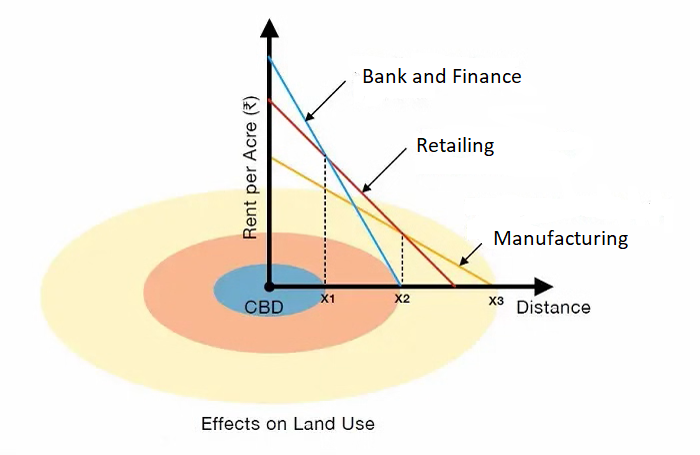
\includegraphics{images/bidrent.png}

The illustration shows three categories: The most expensive rent closest
to the centre is the Bank and finance district, followed by the retail
agglomeration areas and industrial sites furthest away from the central
point. Dental practices are service orientated thus depending on
population density and central activities. Opening hours are relay
outside of office hours. Production cost does not appear to be important
in this case since dentist is a public service. Hence, not dependent of
regular transportation of sales goods. The rent realized by the
landowner is the envelope of the three rent supply curves Capello
(2015). From a Marshallian way of thinking dentists should cluster
somewhere in this pink area to reap maximum sales volume. Other than
locating in the inner circle dentists may also increase their profits
further out in to other retail agglomeration area. The attractiveness
might be high in these places due to economies of scope. As the positive
benefits from the Marshallian agglomeration attributes play out.
Subsequently, increasing profit by trading higher transportation cost
for lower rent. In addition fewer dentists to compete with. The
attendances to break out of the clusters support Hotelling's game theory
of spatial competition which suggests that the spatial monopoly power
provides an incentive for firms to use location as a competitive weapon
to achieve spatial monopoly (\textbf{mccann2013McCann?}).

\textbf{Gravitational models}

The centre attracts firms, people and activities. Furthermore, it
influence the central points in diverse ways such as commuter movements,
disfustion of knowledge, corporations and network and personal
relationship Capello (2015). More-so, they are generated by the
intensity of the flows generated between places Capello (2015). The
gravitational pull to a place of interest for a dentist will determine
how much sales can be generated by locating there. Several locations can
then be measures against each other to determine profit maximisation.
These models has the potential to measures the future attractiveness of
a place. Changes in infrastructure such easier access to a place might
change the attractiveness of a place or move the flow of people. An
example of this could be Rogfast, improving the connection between
Haugalandet and Stavanger. Subserviently, increasing the gravitationally
pull between the two places. Furthermore, The model uses population and
distance to measure the attractiveness and relations between two places
Capello (2015). Rogfast might move the population of Haugesund further
south and a new town centre might occur competing with other retail
clusters in years to come. On the other hand the flow of people towards
Raglamyr might increase until the potential new centre place has grown.
These models have predictive capacity and can be used to estimate the
potential impact. In particular, location of new productive activity in
an area Capello (2015). For instance predict where to build a shopping
centre Capello (2015). A new shopping centre further south in Haugaland
or expansion of excising retail agglomeration areas might be of
interest. As a result of increased population. By taking these factors
in to account dentist could predict the most profitable locations in
years to come by predicting the amount of people that will move from one
city to another or tow different points of interest within a city.

\textbf{Retail Agglomeration and Economies of Shopping Centres}

Town and cities have long had shopping districts in which stores are
concentrated. To some extent such centre points were the result of
uncoordinated store-location decisions Brueckner (2011). Nevertheless,
not coincidentally according to Hotelling's theory (1929). He describes
the concentration of retail stores by a market desire to create a Nash
equilibrium. At this point all retailers expected sales maximisation
outcome cannot be improved by changing position. Contradictory to the
assumption that consumers will shop at the nearest retailer, they are
willing to travel significantly further to reach certain central places.
Marshall (1920) points out another explanation for this in his seminal
work on agglomeration. That being,intra-industry knowledge spillovers as
mechanisms leading to formation of industry cluster Nielsen et al.
(2021). In this case the dental industry information spillovers are
bounded in geographical space. Hence, the need to locate in close
proximity. That being the latest equipment, in order to work faster or
the right personnel to attract more patients. Another way to drive sales
in this area could be by dentist specialisation and patients referrals
between dentists.

Another important externalities expressed in Marshall (1920) theory is
market transactions. Whereas, geographical proximity reduces transaction
cost through several mechanism Nielsen et al. (2021). The market
transactions can be extended to the endogenous location of specialized
human capital Nielsen et al. (2021). ``It is well known among economists
and other social scientists that large cities have disproportionately
large shares of highly educated workers, and the trend has been growing
in recent decades.'' Baker (n.d.) Presumably, larger cities would then
be more attractive to dentists in terms of cost and quality of
specialised labour in smaller towns. Especially, those trying to achieve
spatial monopoly end up loosing profit by overpaying for labour or in
worst case scenario not finding enough dentists labour and end up
compromising on quality. In both cases growth potential would be
compromised.

Marshal also points out the competition within the geographical
location. Hence, the marketplace and business districts give consumers
low search and switching costs Capello (2015). The fact that owners of
stores seem to prefer highly concentrated shopping. More-so, it suggests
that the sales volumes outweigh the loss attributed to greater price
competition.

\textbf{Shopping Malls}

Owners of shopping malls ``orchestrate'' the process of retail
agglomeration that happens naturally in towns and cities Brueckner
(2011). Naturally, the same retail agglomeration and Nash equilibrium
may occur in shopping malls if not more intensely as the shops are in
closer proximity. Furthermore, the potential for more knowledge
spillovers, higher volume of market transaction and more competition.
When retail agglomeration is orchestrated by the owner of a shopping
mall, the strength and direction of such externalities are taken into
account Brueckner (2011). Much so, because the price of rent is
dependent on the overall revenue of a shopping mall. Hence, the owner of
the mall wants to choose the mix of stores and their sizes taking these
externalities, attributes and anchor stores attractiveness into account
Brueckner (2011). The Norwegian retail market for alcoholic beverages is
controlled by the state monopoly. Anchor-stores such as the
Wine-monopoly bring in a higher volume of consumers
(\textbf{lai2013Lai?}). For example, shoppers visiting the Wine-monopoly
in a mall may also visit a clothing store, and even find it beneficial
to use public services at the same time. Nevertheless, they are limited
in numbers and needs government approval. Each municipality must apply
to get the wine monopoly in their area. One of the factors considered in
this process is the death of city centre. A possible reason for this is
so called ``predatory malls'' which are purposely built to overtake the
exciting local market. Perhaps more so if malls cater for cinema,
restaurants, bars and other attributes in conjunction with the city
centre. Not to mention the upper hand of easy road access and free
parking.

\hypertarget{data}{%
\subsection{Data}\label{data}}

\texttt{In\ quantitative\ studies\ this\ section\ provides\ details\ about\ dataset,\ variables,\ instruments\ and\ measurement\ procedures\ used\ in\ the\ study.\ If\ the\ data\ was\ collected\ by\ the\ authors\ this\ section\ will\ describe\ how\ the\ sample\ was\ collected.\ If\ specific\ instruments\ were\ constructed\ to\ collect\ the\ data\ they\ will\ be\ described\ here\ and\ included\ in\ the\ appendix.\ Procedures\ used\ to\ measure\ variables\ are\ often\ described\ in\ sufficient\ detail\ to\ permit\ replication.\ In\ economic\ papers,\ this\ section\ describes\ the\ empirical\ model\ and\ estimation\ strategy\ used\ by\ the\ authors.}

\textbf{Data description}

For this assignment we where provided with different geospatial data in
the geographic information software QGIS to calculate the relationship
of the different variables that might determine firm activity. This
geospatial data included Norwegian commune data which contained the
administrative boundaries of the Communes, presented in the software as
different divisions of lines that distinguish the different commune
boundaries. We where also provided with different point layers, such as
the geometric centers of communes, urban city centers or Central
Business Districts (CBD), all businesses in Norway which are regarded as
dental services, and all Norwegian shopping malls. We where also
provided with a QGIS layer with population density estimates, visualized
with 100x100 raster graphics.

To carry out a more complete data analysis of the influencing factors of
the activity of Norwegian dentist services, we had to collect more data
than what we already had been presented with. We firstly utilized QGIS
to calculate different other statistics and variables. Regarding the
Norwegian shopping malls layer we added the variable ``Wine-monopoly''
as a false/ true variable to determine which Norwegian malls had a hard
liquor store. We added the number of stores which are in each mall, to
use as an estimate for the malls sizes. The malls opening hours have
also been included in this layer. From SSB, we gathered data on the
average municipal sales per inhabitant in retailing for each Norwegian
commune. Lastly we created 2 kilometer buffer zones around dentists and
CBDs to determine population density in these areas.

After calculations in QGIS we transferred our data to RSTUDIO to do the
primary statistical analysis of our data. The data is then merged into
two different data frames. The first one containing Norwegian communes
as the unit of observation, which includes geometric commune centers to
the nearest mall, the retail per capita per commune, the different
commune numbers and the size of the nearest mall, including the true/
false ``Winemonopoly'' variable. The second data frame use dentists as
the unit of observations. This data frame include data on the distances
from CBD to dentists, distances from dentists to the nearest mall,
including variables of the mall size and the ``Winemonopoly'' variable,
different significant accounting figures for the different dentist
businesses, such as total sales revenue and EBIT (Earnings Before
Interests and Taxes).

To obtain a first impression and a simple understanding of our data, we
have decided to make use of scatterplots. The scatterplot presented in
\textbf{?@fig-1} show the relationship of average spending on retail
amongst inhabitants and the distance from geometrical commune centers to
nearest malls, which indicate that most malls are in a 50 km radius of
commune centers, and that Norwegians on average spend between 50
thousand to 120 thousand on retail.

We furthermore have used plots to look at the relationship between the
income of dentist's businesses and the distance from CBDs. The
scatterplot in \textbf{?@fig-2} have some extreme figures of 1 billion+
income which we choose to ignore and deem as outliers, as we notice that
these observations are accounting figures for an entire group of
companies under the same legal name, and not individual companies. By
ignoring these outliers we are then left with the scatterplot in
\textbf{?@fig-3}. This plot shows a tendency of a negative relationship
between the variables, which might suggest that dentists might earn more
closer to CBDs. The last scatterplots we have chosen to calculate is
concerning the relationship of dentists EBIT which is earnings before
interest and taxes, compared to their distances to the nearest shopping
mall in \textbf{?@fig-4}. Just as the previous scatterplot, we also see
here a tendency of a negative relationship between the variables. A
decent number of dentists run at a loss, having negative earnings before
interest and taxes.

\textbf{Empirical Specification}

\textbf{Econometric Approach}

\textbf{Estimation strategy}

\textbf{Analytical framework}

SEDA (Spatial Explanatory Data Analyses)

Spatial data analysis is a rapidly growing area in Statistics Haslett
(1992). The Journal of the statistics society define such data as being
objects in space, which objects have physical location. Furthermore, the
analyses are spatial if these locations are relevant to the
interpretation of the data Haining, Wise, and Ma (1998).

The examination of the data involves the examination of data collected
from q-gis maps;
\texttt{it\ will\ involve\ little\ more.\ Graphical\ techniques\ for\ examining\ such\ maps\ are\ thus\ a\ central\ part\ of\ the\ methodology.\ A\ number\ of\ such\ techniques\ are\ discussed."}
Haslett (1992).

\texttt{What\ data\ are\ used?}

\texttt{What\ has\ been\ calculated?}

\hypertarget{results}{%
\subsection{Results}\label{results}}

\hypertarget{discussion}{%
\subsection{Discussion}\label{discussion}}

\hypertarget{conclusion}{%
\subsection{Conclusion}\label{conclusion}}

\hypertarget{acknowledgements}{%
\subsection{Acknowledgements}\label{acknowledgements}}

\hypertarget{references}{%
\subsection*{References}\label{references}}
\addcontentsline{toc}{subsection}{References}

\hypertarget{refs}{}
\begin{CSLReferences}{1}{0}
\leavevmode\vadjust pre{\hypertarget{ref-brueckner2011}{}}%
Brueckner, Jan K. 2011. \emph{Lectures on Urban Economics}. MIT Press.

\leavevmode\vadjust pre{\hypertarget{ref-capello2011}{}}%
Capello, Roberta. 2011. {``{[}PDF{]}location, Regional Growth and Local
Development Theories,''} January.
\url{https://www.academia.edu/48547951/_PDF_Location_Regional_Growth_and_Local_Development_Theories}.

\leavevmode\vadjust pre{\hypertarget{ref-capello2015}{}}%
---------. 2015. \emph{Regional Economics}. 2nd ed. Routledge.
\url{https://doi.org/10.4324/9781315720074}.

\leavevmode\vadjust pre{\hypertarget{ref-haining1998}{}}%
Haining, R., S. Wise, and J. Ma. 1998. {``Exploratory Spatial Data
Analysis.''} \emph{Journal of the Royal Statistical Society: Series D
(The Statistician)} 47 (3): 457--69.
\url{https://doi.org/10.1111/1467-9884.00147}.

\leavevmode\vadjust pre{\hypertarget{ref-haslett1992}{}}%
Haslett, John. 1992. {``Spatial Data Analysis---Challenges.''}
\emph{Journal of the Royal Statistical Society: Series D (The
Statistician)} 41 (3): 271--84. \url{https://doi.org/10.2307/2348549}.

\leavevmode\vadjust pre{\hypertarget{ref-mccann2013}{}}%
McCann, Philip. 2013. \emph{Modern Urban and Regional Economics}. Second
edition. Oxford University Press.

\leavevmode\vadjust pre{\hypertarget{ref-nielsen2021}{}}%
Nielsen, Bo Bernhard, Christian Geisler Asmussen, Cecilie Dohlmann
Weatherall, and Ditte Håkonsson Lyngemark. 2021. {``Marshall Vs Jacobs
Agglomeration and the Micro-Location of Foreign and Domestic Firms.''}
\emph{Cities} 117 (October): 103322.
\url{https://doi.org/10.1016/j.cities.2021.103322}.

\end{CSLReferences}



\end{document}
